\section{Problem Formulation and Information Contract}
\label{sec:problem}

\subsection{Kinematic model and fixed-period follower}

We consider one translational or rotational coordinate with state $x=(p,v,a)$ and control $j$,
\begin{equation}
 \dot p=v,\qquad \dot v=a,\qquad \dot a=j,
 \label{eq:third-order}
\end{equation}
subject to symmetric bounds
\begin{equation}
 \abs{v(t)}\le V,\qquad \abs{a(t)}\le A,\qquad \abs{j(t)}\le J.
 \label{eq:bounds}
\end{equation}
The control period is $T$. At tick $k$, the follower initializes the OTG from the state produced at the end of the preceding tick, supplies a target state, commits one period of the returned trajectory, and repeats. The generator may compute a trajectory whose free duration exceeds $T$; our mechanism analysis nevertheless inspects exactly what is executed on $[kT,(k+1)T]$.

Let $P[k]$ denote the scheduled position at time $kT$. A constant-speed schedule satisfies
\begin{equation}
 P[k+1]-P[k]=\vref T.
 \label{eq:constant-schedule}
\end{equation}
The operational distinction is not whether the position is current or one step ahead; it is which complete state accompanies that position. We study three target contracts:
\begin{align}
 \Ponly &: \targetstate_{k+1}=(P[k+1],0,0), \label{eq:p-contract}\\
 \PV &: \targetstate_{k+1}=(P[k+1],\widehat V[k+1],0), \label{eq:pv-contract}\\
 \PVA &: \targetstate_{k+1}=(P[k+1],\widehat V[k+1],\widehat A[k+1]). \label{eq:pva-contract}
\end{align}
For constant motion, the matched values are $\widehat V[k+1]=\vref$ and $\widehat A[k+1]=0$. Thus matched PVA carries no additional physical information beyond matched PV in that special case; it is retained as a negative control, not dismissed for general motion.\claimtag{C8}

\begin{figure*}[t]
 \centering
 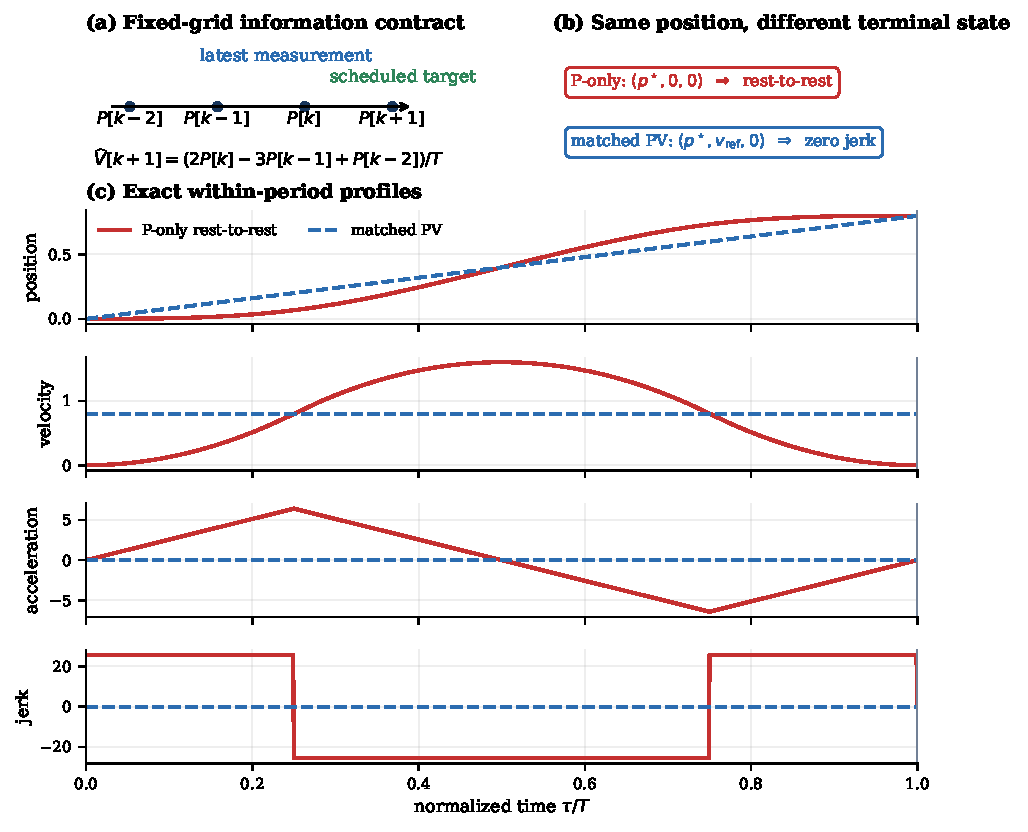
\includegraphics[width=\textwidth]{figures/generated/fig1_mechanism_profiles.pdf}
 \caption{Mechanism and information contract. (a) At tick $k$, $P[k+1]$ is an already scheduled target; measurements are available only through $P[k]$. (b) Identical position targets encode different terminal states. (c) A representative feasible P-only transfer reaches the correct endpoint after a rest-to-rest pulse, whereas matched PV admits constant velocity and zero jerk. The profiles are analytic normalized examples, not measured robot signals.}
 \label{fig:mechanism}
\end{figure*}

\subsection{Scheduled target versus future measurement}

The indexing in \cref{eq:pv-contract} can otherwise invite a noncausal interpretation. We define the information available when constructing the target for interval $[kT,(k+1)T]$ as
\begin{equation}
 \mathcal I_k=\{P[k+1]\text{ scheduled};\ P[k],P[k-1],P[k-2]\text{ available}\}.
 \label{eq:information-set}
\end{equation}
The semicolon is important. The target scheduler has already made $P[k+1]$ available, but no measurement after time $kT$ is observed. A predictor that reads only the history through $P[k]$ is causal under this contract even though its output is associated with the scheduled target at $k+1$. This is the timeline shown in \cref{fig:mechanism}a.

Our fixed-grid \FutureOOne{} velocity target is
\begin{equation}
 \widehat V[k+1]=\frac{2P[k]-3P[k-1]+P[k-2]}{T}.
 \label{eq:future-o1}
\end{equation}
The name describes the one-step target association used by the implementation; it does not mean that $P[k+1]$ is used as a future measurement. Startup samples use the explicitly reported fallback in the experiment specification. E17's irregular-timestamp replay deliberately rejects \cref{eq:future-o1} when the prediction horizon is not exactly one nominal step, rather than silently applying a fixed-step formula to a different contract.\claimtag{C5}\claimtag{C13}

\subsection{Mechanism metrics}

Endpoint position error is insufficient to identify \stopandgo. For every committed interval, the experiment reconstructs the exact piecewise-constant-jerk profile returned by the solver and evaluates it within the period. The primary mechanism readouts are: rest-to-rest pulse fraction, endpoint-stop fraction, stop-and-go event rate, velocity ripple normalized by $\abs{\vref}$, the lower tail of within-period $\abs v/\abs{\vref}$, and the fraction of cycles containing near-zero velocity. A profile-exact flag records whether the candidate matches the preregistered invariant profile within numerical tolerance. Constraint violations, fallbacks, solver failures, and incomplete cycles are guardrails.

For a constant reference, normalized velocity ripple is the range of the exact within-period velocity divided by $\abs{\vref}$. It is zero for the constant-velocity continuation and positive for an acceleration--deceleration pulse. The near-zero and endpoint-stop metrics distinguish a profile that merely varies around $\vref$ from one that actually stops. E15 and E16 therefore do not infer the mechanism from RMSE or from a target field alone.

\subsection{Recorded waveform metrics}

The recorded case uses raw-time position RMSE after a fixed startup exclusion, integer cross-correlation lag on the 10 ms grid, and a local quadratic sub-sample refinement. We call both lag quantities \observedlag{} because they describe alignment between two waveforms. They do not measure computation time, communication delay, or closed-loop wall-clock latency. Target projection and kinematic limit checks are scientific guardrails. Per-cycle execution time and deadline misses are reported separately as offline-host diagnostics.

The recorded input contains \RecordedSampleCount{} samples over \RecordedDuration. It is one trajectory on one axis, not a population of tasks. Comparisons within A04 and A06 use the same velocity-limited waveform; we do not form causal performance ratios between the current-online baseline and a candidate produced from a different input waveform. These restrictions define the scope of the recorded case study before any result is examined.\claimtag{C9}\claimtag{C10}

